\documentclass[preprint,12pt]{elsarticle}
\usepackage{graphicx}
\usepackage{amssymb}
\usepackage{hyperref}

\journal{ITEC876}

\begin{document}

\begin{frontmatter}

\title{Reproducing StarGAN}

\author{Reuben Francis, Sanjay Adhikari, Gautham Meenakshisundaram, Bhavana Ramanna}

\address{Macquarie University}

\begin{abstract}
A research can be reproducible when published results can be replicated using data, code, and paper provided by the authors and being able to reach the same results as claimed. Reproducibility, so as to being very close to replicability, is the act of repeating a methodology to prove correctness, or even reaching similar conclusions to the required result. These are the basis of tackling an empirical research\cite{gitbook_bot_2018_1212538}. This isn't just corroboration but also serves as an exposure of research workflows and transmission of knowledge. 
\end{abstract}

\begin{keyword}
Empirical Research \sep Reproducibility

\end{keyword}

\end{frontmatter}

\section{Source Paper Description}
\label{S:1}

Our reproducible research shouldn't be too complex or unmanageable, breaking down the possible factors that give in to reproducibility is important. Selecting a research paper requires understanding of its impact, the overall setup that explains workflows, data management and finally the individual steps for reproduction and required resources. 

One such paper is the StarGAN multi-domain image-to-image translator \cite{StarGAN2018}. Existing image translators have limited scalability and robustness when it comes to multiple domains, different models needed to be built for every pair of image domains. The StarGAN out-rules this issue with just a single model that simultaneously trains on multiple data-sets with different domains. The architecture is flexible in translating any input image to a desired target domain. The paper performs an empirical demonstration of its effectiveness on facial attributes. 

\subsection{Evaluation Framework}

The research paper carries out its evaluation on two sets of data, in which we are only interested in one of them. They compared their model to the baseline models, DIAT and CycleGAN based on single and multi-attribute translations. The base models as said, require multiple cross-domain models for all possible attribute pairs. The qualitative evaluation shows how well the model provides a higher visual quality translation result on test images when compared to baseline models. The researchers mention it's flexibility being universally applicable across domains of facial images being the main reason.

Another evaluation carried out by the researchers is a quantitative survey study that used Amazon Mechanical Turk (AMT) to assess single and multiple attribute transfer tasks. The surveys were handed over to Turkers who chose images based on realism, quality of transfer and degree of image's original identity while comparing them with other models. Each user study had 30 to 40 logical questions which was validated by 146 Turkers for single transfer and 100 for multiple transfer domain.

Based on these frameworks, the quantitative results produced very satisfactory results,  when compared with the baseline models. StarGAN outvoted the others for its degree of attribute transfer, especially with respect to multi-attribute changes. As mentioned in the qualitative analysis, the proposed model can handle any attribute changes just by generating a target domain label while training. 

\subsection{Justification}

Continuing on factors that make a research paper reproducible, justification does play a role. Under-powered study in this case is a possible issue, if an analysis detects an effect, the under-powered study in the first place would be too meager to reliably indicate whether or not the effect exists. CORE rankings or Google Scholar discipline rankings can be used to justify the quality of a research paper. If not, even the number of citations counts as a quality check. As per Google Scholar, our paper published in the year 2018 has been cited 508 times. Figure \ref{fig:cite}, is a screenshot of the citation count on Google Scholar of StarGAN paper.\cite{StarGAN2018}. The code for the paper is readily available on GitHub\footnote{GitHub link: \url{https://github.com/yunjey/stargan}.} provided by the researchers themselves. 

\begin{figure}[ht]
\centering
\includegraphics[width=1.0\linewidth]{citation.png}
\caption{StarGAN in Google Scholars}
\label{fig:cite}
\end{figure}

\section{Description of original dataset}
\label{S:2}

Reference to Section \ref{S:1}, we focus on one of the two mentioned data-sets used in the paper, CelebA and RaFD. The latter, Radboud Faces Database (RaFD)\cite{RaFDdataset} is a facial dataset containing different emotional expressions. It however isn't freely available and has a user agreement\footnote{Database request: \url{http://www.socsci.ru.nl:8180/RaFD2/RaFD}.} and has therefore not been worked on. 

The former stands for CelebFaces Attributes (CelebA)\cite{liu2015faceattributes} is freely available online\footnote{Dataset URL: \url{http://mmlab.ie.cuhk.edu.hk/projects/CelebA.html}.} and contains 202,599 face images of celebrities, where each of them are annotated with 40 binary attributes. The initial size is resized from $178\times218$ to $128\times128$. Randomly selected 2000 images are the test set and remaining are part of the training set. From the mentioned 40 attributes, we only use seven domains using the following five attributes : hair color (black, blond, brown), gender (male/female), and age (young/old). Figure \ref{fig:CelebA} shows a snippet of the original CelebA data. 

\begin{figure}[ht]
\centering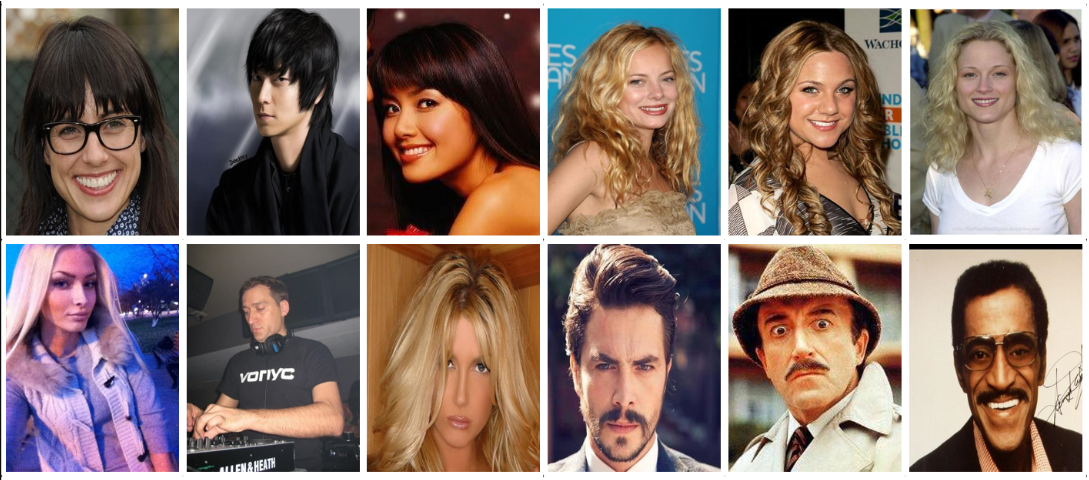
\includegraphics[width=0.7\linewidth]{CelebA.png}
\caption{Snippet of CelebA dataset}
\label{fig:CelebA}
\end{figure}

\section{Replication of original work}
\label{S:3}

Research being replicable is closely related to the idea of empirical generalization. The tools are made available to allow us duplicate the results of the research, maybe even extend it. Before doing so however, there needs to be a good plan that can rectify and notice necessary changes before hand. Our goal is to replicate the StarGAN model and make sure it runs as said with the given data. The paper focuses on comparing the proposed model with baseline models, our reproduction however doesn't do so, no baseline models are replicated. The standalone model is qualitatively evaluated based on human perseverance of what high visual quality translations of image looks like while keeping the source research paper as a standard measure. This evaluation is backed-up with quantitative analysis, that similar to the paper, performs a user study in a survey format.

\subsection{Issues of original work}

The source code mentioned in the paper works just as mentioned in the repository read-me guide. The code is written in python with PyTorch as dependency. Command line arguments are needed to run the python files with a list of attributes that mention details like type of dataset, image size, facial attribute list, directory locations, etc. Since python code and Unix commands were needed, creating a jupyter notebook on Google Colaboratory seemed easier. The following issues are addressed as follows:

\begin{itemize}
\item Making the data available required a shell command to be run that would download the dataset from a server, this however resulted in long process time and some image files being corrupted. 
\item The model took too long to train (approximately 10 hours to train only 30\% of the model), and training with a smaller subset of data gave a badly trained model despite changing hyper-parameters.
\item The repository included a checkpoint that however demanded a need to copy, move, delete, zip and unzip huge files, extending runtime. 
\item New PyTorch update required a lot of libraries, functions and packages to be updated. 
\item The approach didn't seem user friendly when dealing with new dataset. 
\end{itemize}

\subsection{Resolving issues}

The main driving factor of the issues in original work was the need to version change PyTorch in order to keep up running and also exceeded runtimes for data transferring and downloading. Having to change the reference repository seemed necessary, and GitHub happened to have a Tensorflow replicated implementation of the project, rated second to the original work. This repository\footnote{GitHub link: \url{https://github.com/taki0112/StarGAN-Tensorflow}.}, had simpler command line arguments and the CelebA dataset downloaded without an issue. The checkpoint this time however, was present in an external link that needed to be mounted by the drive and the need to move, copy, delete, zip and unzip files around still persists.

These issues were all solved by pushing the necessary changes after getting the environment ready with necessary files to a personal repository\footnote{Github link: \url{https://gitlab.com/reubenbf/stargan-tensorflow/}.}. This approach reduced the code size drastically and made it much easier to use. Figure \ref{fig:StarGAN} is the resultant image translations by the StarGAN model based on the facial attributes.

\begin{figure}[ht]
\centering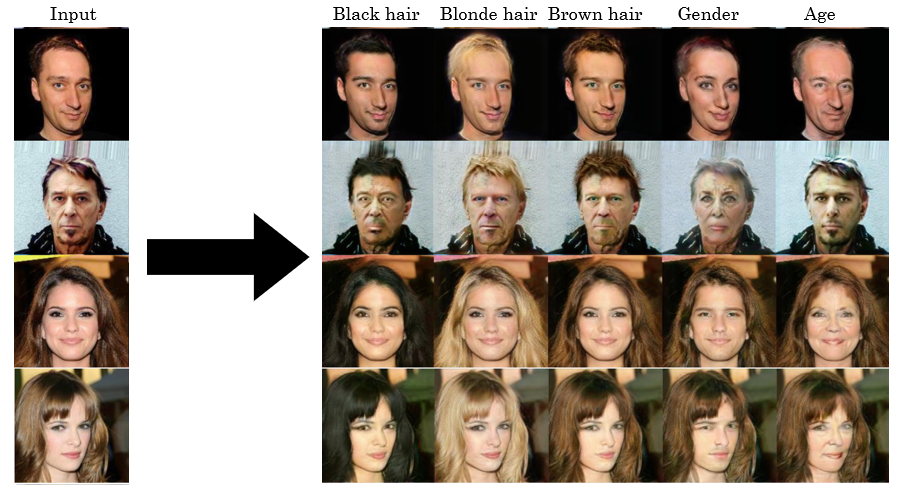
\includegraphics[width=0.7\linewidth]{StarGAN.png}
\caption{Image-to-image translation results on the CelebA dataset. The first row show input images while the remaining columns are images generated by the StarGAN. The images are generated by a single generator network.}
\label{fig:StarGAN}
\end{figure}

\section{Construction of new data}
\label{S:4}

Scientifically, reproducibility is important to help the reproducibility crisis. Consequences of this issue however can be aided with replicability, the ability to replicate a research paper with the same code and achieve similar enough results and graphs in a different set up. The data used could be downloaded from a public repository, re-generated/re-simulated or in our case reproduced by raw extraction of data by certain techniques. 

We've established two scenarios of constructing new data; extracting raw bulk images from a common source and later cropping them to form a set of facial images. This method follows a brute-force mannerism of data construction, a slightly naive approach to collecting required new datasets.

\subsection{Wikipedia API}
Making use of Wikipedia's huge database makes it one of the hubs for data scraping, in our case, image data extraction. This has been made easy thanks to the Wikipedia API which is a Python library that helps access and parse data from the website; including image extraction which however isn't a direct 'image downloader'. The 'images' list of the WikipediaPage object present in the Wikipedia library is a list of image URLs which can be used to fetch images from a Wikipedia page. This list could be passed to the urllib library that has the urlretrieve function which helps download the images to the working directory with respect to its URL.

Resorted to using “List of musicians”\footnote{Wikipedia link:\url{https://en.wikipedia.org/wiki/Lists_of_musicians}.} as the main page, with which we iterate through links present in the page and sub-links of each of these pages were used as query-terms for the WikipediaPage.image object which is later passed to the urlretrieve function. Figure \ref{fig:WikiExtract} explains how the query-terms are produced. 

\begin{figure}[ht]
\centering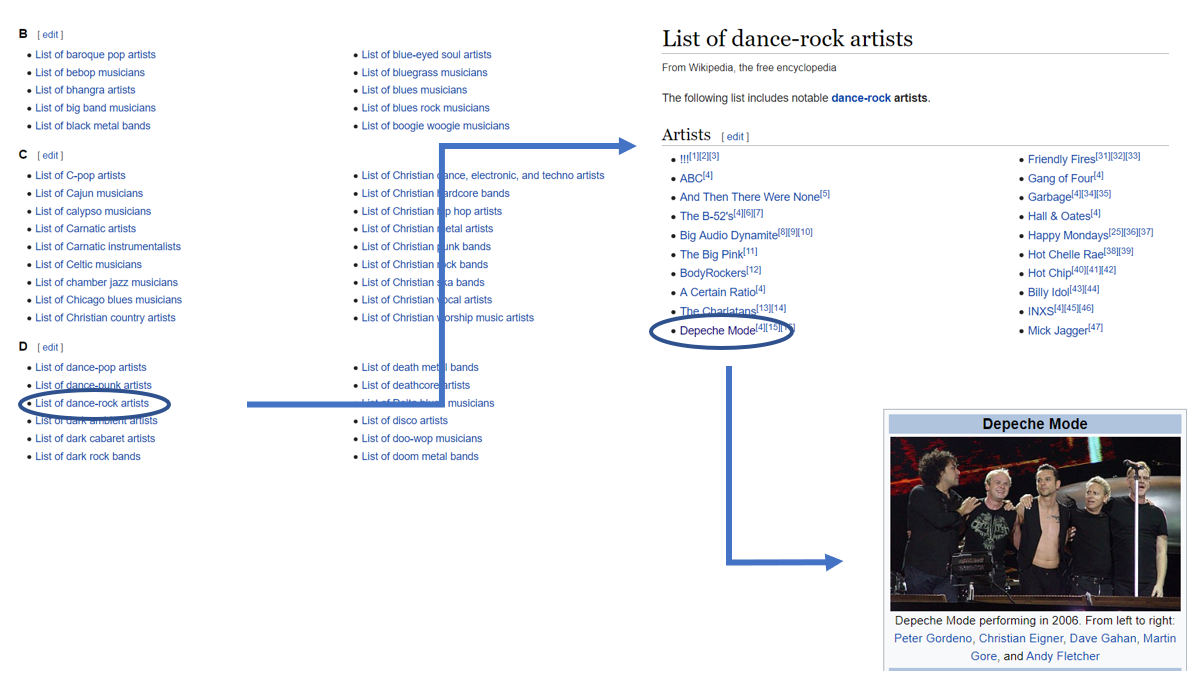
\includegraphics[width=0.5\linewidth]{wikipedia_extractor.png}
\caption{Simple Wikipedia main-page to link to sub-link to image procedure flow}
\label{fig:WikiExtract}
\end{figure}

This is a very raw approach of collecting images since the sub-links of the main-page are expected to be images of artists or bands, this however is not always the case. Some links lead to articles with completely irrelevant sub-links resulting in irrelevant data, images that wouldn't have faces in the first place, this can be described in Figure \ref{fig:WikiExtractIssue}. The code for extraction as well needs to be manually stopped since the sub-link iterate almost endlessly. 

\begin{figure}[ht]
\centering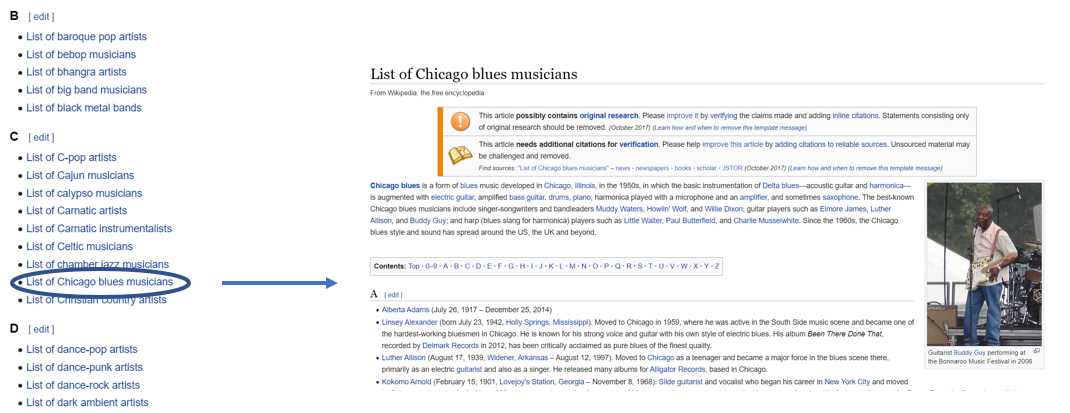
\includegraphics[width=0.7\linewidth]{wikiextract_issue.png}
\caption{Wikipedia sub-link query issue, here terms like 'blues','Chicago', 'electric guitar' and many others would also pass through the image object}
\label{fig:WikiExtractIssue}
\end{figure}

\subsection{YouTube Video Frame Screenshot}
YouTube is another good example of a data scraping hub. Inspired by a GitHub repository 'Face Database Creator'\cite{frc}, our code helps extract a set number of random frames from top ten search results for a given term-query. The search terms used are based on videos that could possibly have potential faces that could be present in the random frames. Figure \ref{fig:Youtube} gives an example of the extracted images produced.

\begin{figure}[ht]
\centering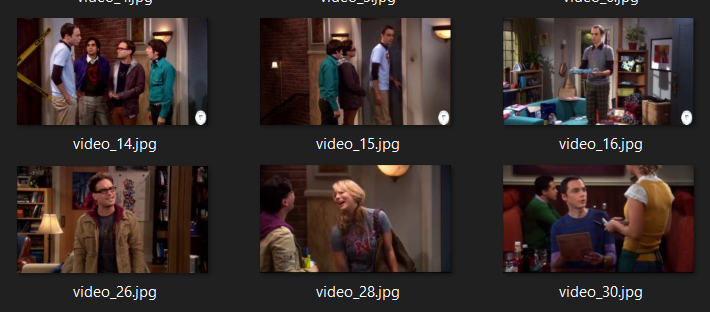
\includegraphics[width=0.7\linewidth]{yt.png}
\caption{Screenshot of random frames extracted from videos with search query 'big bang theory'}
\label{fig:Youtube}
\end{figure}

\subsection{Face Cropper}

The images extracted by the methods mentioned have their own flaws since the technique of approach is naive, the images aren't all that necessary unless an acceptable enough 'face image' can be further extracted, This is done by the face cropper called Autocrop\footnote{GitHub link: \url{https://github.com/leblancfg/autocrop}.} which once installed uses simple command line arguments and user friendly options to resize image, add padding, etc. 

Here, the images generated by the Wikipedia API and the YouTube video frame grabber are treated together as new dataset that is placed in a common folder called 'pics', the autocrop runs on each of these images and crops the images with faces as needed and places them on 'crop' folder while images with no facial features or faces not detected by the program are saved in the 'reject' folder. The finalized cropped images happen to have few ‘non-face’ images but is fairly clean enough. Figure \ref{fig:Cropped} gives a clear example of the final images after being cropped.

\begin{figure}[ht]
\centering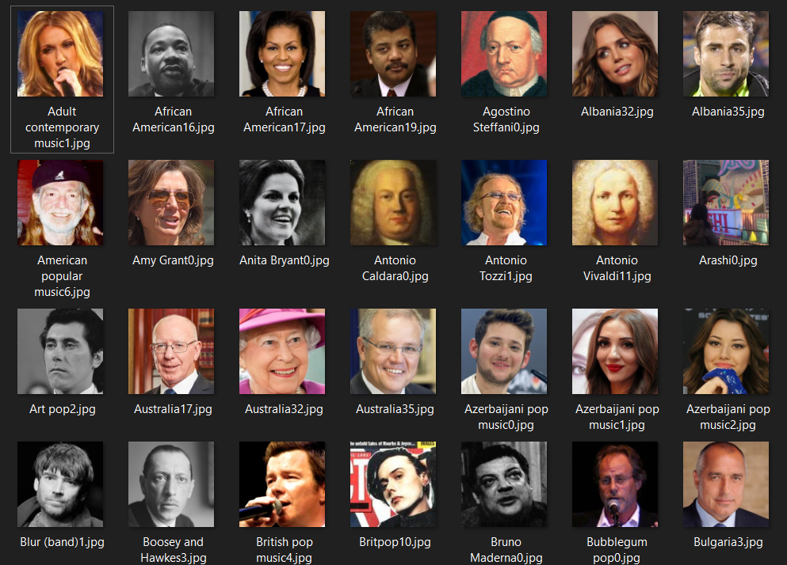
\includegraphics[width=0.7\linewidth]{cropped.png}
\caption{Screenshot of cropped images from Wikipedia and YouTube}
\label{fig:Cropped}
\end{figure}

\section{Results on new data}
\label{S:5}

The custom new dataset is a collection of cropped Wikipedia and YouTube still frame images which now act as imitations to the CelebA dataset and tested to see whether they are able to produce similar results as to the original dataset, justifying claims about the StarGAN model. Having to train a new model would require a lot of new data as well as annotating each of these images with their individual 40 attributes. The changes along with addition of new data have been added to another repository \footnote{GitHub URL:\url{ https://github.com/snj-adhikari/stargan_dataset}.} for ease of use.

To understand the working, an input $128\times128$ image is given to the StarGAN model trained on the CelebA dataset with the five attributes mentioned in Section \ref{S:2}, the output is a series of five horizontally placed $128\times128$ images ($640\times128$ image), Figure \ref{fig:StarGAN_new} is a snippet of our results. Here, each hair color has its own attribute value while however gender and age are binary indications. The model therefore checks for an attribute description for an image to flip the gender and age factor while however, our test images with no annotations are guessed by the model itself and flipped to its counterpart. These images are evaluated with the same framework mentioned for original data.

\begin{figure}[ht]
\centering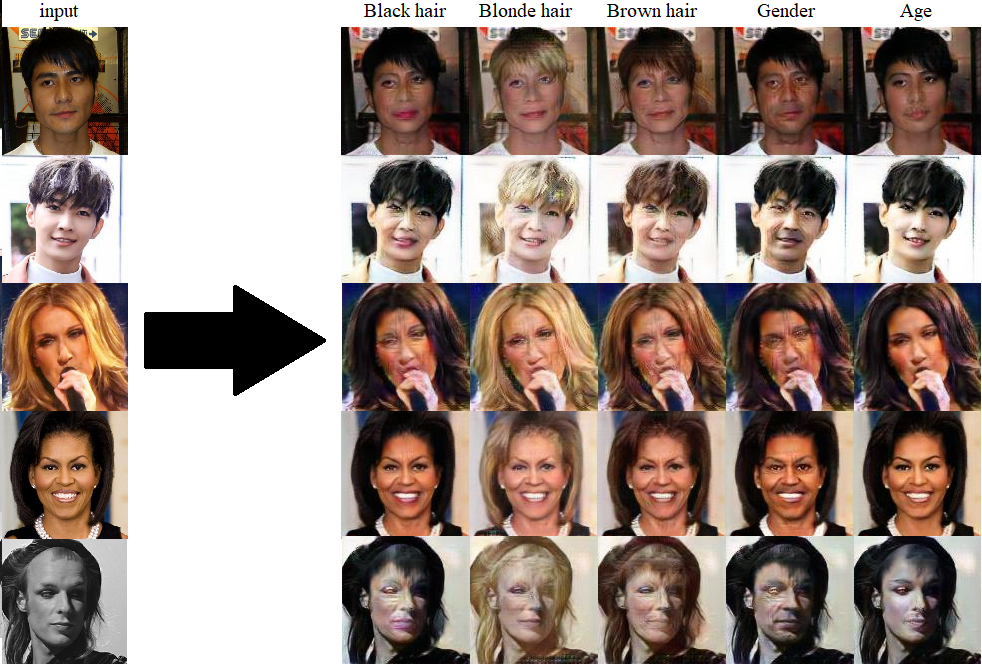
\includegraphics[width=0.7\linewidth]{StarGAN_newdata.png}
\caption{StarGAN model run on new dataset, the first row is the input data and the following rows are images translated by the model based on their attribute}
\label{fig:StarGAN_new}
\end{figure}

A qualitative evaluation would require a baseline model to compare with, which however is not part of our finding as seen in Section \ref{S:1}. The generated images would be visually 'good' which is a very biased conclusion. Quantitatively however, a similar user survey can be performed. We've planned to use Google Forms for surveying the 'fake' images and receiving feedback as a form of evaluation. Feedback not being descriptive but however a questionnaire with a scoring system to evaluate how ‘good’ an image is keeping in mind factors like realism, quality of transfer and degree of image's original identity scaled from 0 to 5 and also comparative multiple choice questions that evaluate the difference between the generated with real images. We design a camouflage percentage for each attribute that shows how well a generated image is 'hidden' whilst other real images, a value that is a ratio of counts outvoting the fake image to all the votes. Table \ref{table:Avg_score} shows the results of the average scores obtained from each of the attributes used while Table \ref{table:Camou} shows camouflage percentage for each attribute.


\begin{table}[ht]
\centering
\begin{tabular}{l l}
\hline
\textbf{Attributes} & \textbf{Average Score}\\
\hline
Black Hair & 4.05 \\
Blonde Hair & 3.83 \\
Brown Hair & 3.66 \\
Gender & 2.83 \\
Age & 2.55 \\
\hline
\end{tabular}
\caption{Table indicating an average score given to translated images based on their attribute transformation.}
\label{table:Avg_score}
\end{table}

\begin{table}[ht]
\centering
\begin{tabular}{l l}
\hline
\textbf{Attributes} & \textbf{Camouflage Percentage}\\
\hline
Black Hair & 83.7\% \\
Blonde Hair & 81\% \\
Brown Hair & 78.3\% \\
Gender & 75.6\% \\
Age & 62.1\% \\
\hline
\end{tabular}
\caption{Table indicating an camouflage percentage given to translated images based on their attribute transformation. For example, 83.7\% voters couldn't recognise the generated black hair image when compared with real black hair images}
\label{table:Camou}
\end{table}

\begin{figure}[ht]
\centering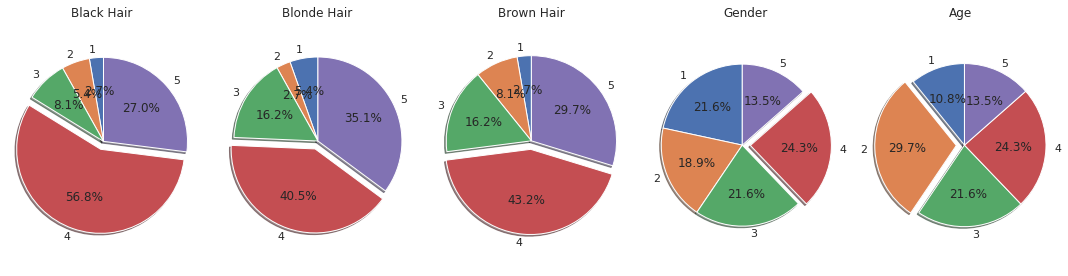
\includegraphics[width=0.7\linewidth]{survey_1_summary.png}
\caption{Survey - Percentages of ratings observed for the transformations produced by StarGAN on 5 attributes.}
\label{fig:summary_1_survey}
\end{figure}

\begin{figure}[!htb]
\centering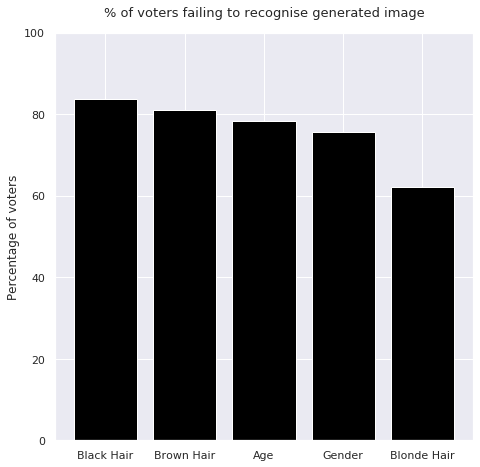
\includegraphics[width=0.7\linewidth]{accuracy_evaluation.png}
\caption{Survey 1 - Percentage of voters finding the generated image in a set of images.}
\label{fig:accuracy_survey}
\end{figure}


Figure \ref{fig:summary_1_survey} shows a series of pie charts for each attribute. Each pie chart shows a ratio of ratings from 1 to 5 (color coded) on the survey by each voter. Figure \ref{fig:accuracy_survey} shows the voters failing to realise the difference between the fake and real images.



\section{Reflections}
\label{S:6}


When testing the results with our new dataset, the model fails to give results as claimed by the paper. The survey proves that the conversion is visually appealing but when compared with the original images, doesn't hold up. One of the main disadvantages is the new data created with our naive technique doesn't hold a guarantee image data, the cropper passes some of the extracted images as faces (when they clearly aren't) and the StarGAN is forced to translate these 'senseless' images. 

\begin{figure}[ht]
\centering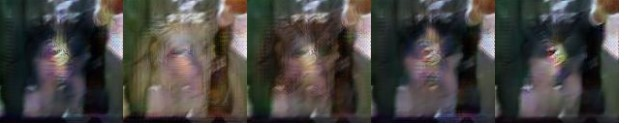
\includegraphics[width=0.7\linewidth]{non_face_image.jpg}
\caption{Example of bad quality image generated with StarGAN.}
\label{fig:StarGAN_bad}
\end{figure}

Figure \ref{fig:StarGAN_bad} shows how the StarGAN model tries to replicate raw 'faceless' images produced by the cropper. This however only occurs rarely since the cropper passes a majority of the face images as needed but throws in a few exceptions that at times gives results as shown.

Despite the cropper resulting in very passable facial images, the result output of StarGAN is still not good as seen in Figure \ref{fig:StarGAN_yt}.

\begin{figure}[ht]
\centering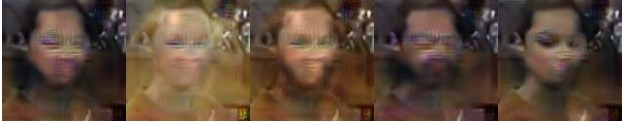
\includegraphics[width=0.7\linewidth]{preety_bad.jpg}
\caption{Bad quality output of StarGAN for Sheldon's images from a YouTube video.}
\label{fig:StarGAN_yt}
\end{figure}

The original CelebA dataset contains images each annotated with 40 binary attributes, this helps the StarGAN model recognise the input image despite being a test process. The model has a pre-knowledge of what it has and makes it easier for it to translate to its required result. Therefore, for an image annotated as a black haired woman, the model now knows that the black hair conversion doesn't need work and the gender flip needs to be a male. Pre-annotating our new dataset however, is one of our huge limitations in terms of time and resources. Figure \ref{fig:StarGAN_tagged} is an example of one of the five sample annotated images from our images cropped and extracted from YouTube.

\begin{figure}[ht]
\centering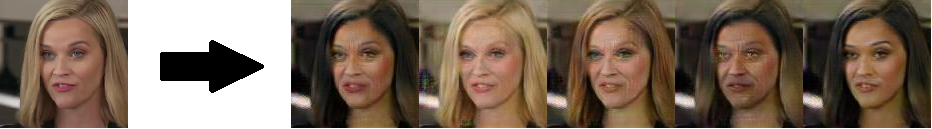
\includegraphics[width=0.7\linewidth]{StarGAN_tagged.png}
\caption{Sample output of an annotated image extracted and cropped from YouTube}
\label{fig:StarGAN_tagged}
\end{figure}

A possible explanation for the higher failure of conversions is the fact that the images have been trained on a different dataset and tested on raw images of different sources. Training a new model with a combination of both the extracted images (Wikipedia and YouTube) which are cropped as need, while also annotating them properly with the 5 needed attributes could possibly make us understand the rate of conversion and whether the model could give out good results or need hyper-parameter adjustments.

There were some limitations when evaluating the output images which are as follows. 

\begin{itemize}
\item Since, these are machine generated images, it is harder to evaluate whether the images are acceptable for human eye.
\item The output images should be validated by human annotation.
\item The use of human annotation platforms such as Amazon Mechanical Turk due to cost and time limitation.
\item Google Forms distributed to a small sample size had to be considered for evaluating the output images.
\item The limitation of google forms is that the results are not reliable as the respondents do not have subject matter knowledge.
\item There is also a possibility of  people responding to the questionnaire with inaccurate or biased ratings.
\end{itemize}
\hfill \break
Possibility of better results could have been achieved if 
\begin{itemize}
    \item Annotation was done for  our images with binary labels 
    \item Training and testing was done  with our own new dataset rather than CelebA.
    \item Better resolution images were extracted in our dataset rather than images with non existent faces.
    \item Black \& white images of Wikipedia data was removed, as StarGAN has difficulty in dealing with those images. 
    \item More face image data is available that could help in training or testing StarGAN.
\end{itemize}

Having noticed our limitations, we have tried producing a new and improved survey that simulates the original by putting up a scoring system not for every individual attribute but the models achievement as a whole. All five images are judged under a common ground, multiple such images with a single scoring system questionnaire format. The selection of images in the existing survey are not randomized but carefully selected images. The existing survey include the bad results mentioned above, along with the poorly translated 'non-face' images as well. Figure \ref{fig:Survey_update} shows the results of the new unbiased survey.

\begin{figure}[ht]
\centering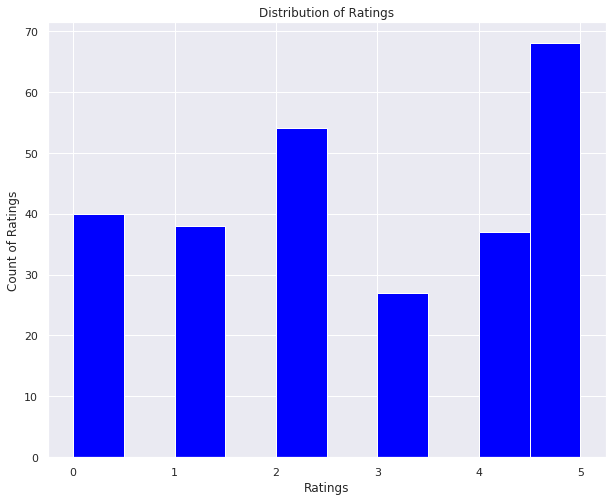
\includegraphics[width=0.7\linewidth]{survey_2_summary.png}
\caption{Histogram of the new survey showing frequency counts of ratings observed in each question. The ratings peak at 5 and 2 suggesting how some images translate good while a good number of them are bad which is a justifiable conclusion}
\label{fig:Survey_update}
\end{figure}

Concluding on our empirical research, we do notice that replicating the original paper did have its flaws, having to make changes for ease of use and reproducability further proves the existence of the reproducability crisis. The paper is reproducable at a certain extent but for when approached naively doesn't give good enough results. Helping this further would be the creation of this research paper, reporting and publishing this methods and interventions explicitly and transparently and fully to allow for replication does contribute to resolve the crisis. Our GitHub repository \footnote{GitHub link: \url{https://github.com/snj-adhikari/ITEC876-Final_Report}.} also consists of the latex code used to write this research paper.

%% References with bibTeX database:

% \bibliographystyle{model1-num-names}

%% New version of the num-names style
\bibliographystyle{model1-num-names}
\bibliography{sample.bib}

%% Authors are advised to submit their bibtex database files. They are
%% requested to list a bibtex style file in the manuscript if they do
%% not want to use model1-num-names.bst.

\end{document}